\chapter{Architectural Design}
\section{Overview: high-level components and interactions}

As anticipated in the previous chapter, the architecture selected for the design and development of the system is the three-tier architecture.

This architecture allow us to split the implementation into three layers:
\begin{enumerate}
	\item Presentation: is the mobile application that will be used by the final users. It allows all the interactions with the system and will also be used as a communication endpoint for the notifications.
	\item Application: is the backend of the system, all the business logic and the various connections between the system and the external services are implemented here.
	\item Data: is the layer responsible to expose connectivity interfaces from the database. It will be a DBMS.
\end{enumerate}
All the layers communicate in a linear way: the Presentation one interacts only with the Application layer, the same as the Data layer. With this architecture the presentation and the Data layers have no direct communication path, this allow to develop all the business logic only in the Application layer.
Other advantages of using this architecture are that the various layers can be developed with different technologies and that they can be duplicated and differentiated (i.e. there can be multiple presentation layers that interact with the same application layer)

The main reasons behind the choice are:
\begin{itemize}
	\item We are not the producer of the data
	\item We need to integrate different external services
	\item Separate the business logic from the data to:
	\begin{itemize}
		\item Allow a parallel development with multiple teams specialized in the single tiers
		\item Allow to use different technologies for the different tiers
	\end{itemize}
\end{itemize}


\begin{figure}[h]
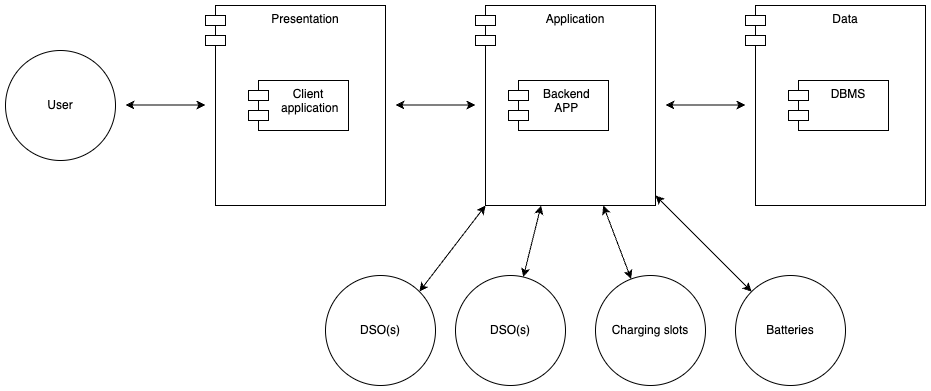
\includegraphics[width=\textwidth]{component_diagrams/overview}
\caption{Overview of the chosen three-tier architecture with actors}
\end{figure}

\clearpage

\section{Component view}
The following schema shows all the main components and interfaces of the system. Later on you will find the details of each component.


\begin{figure}[h]
\centering
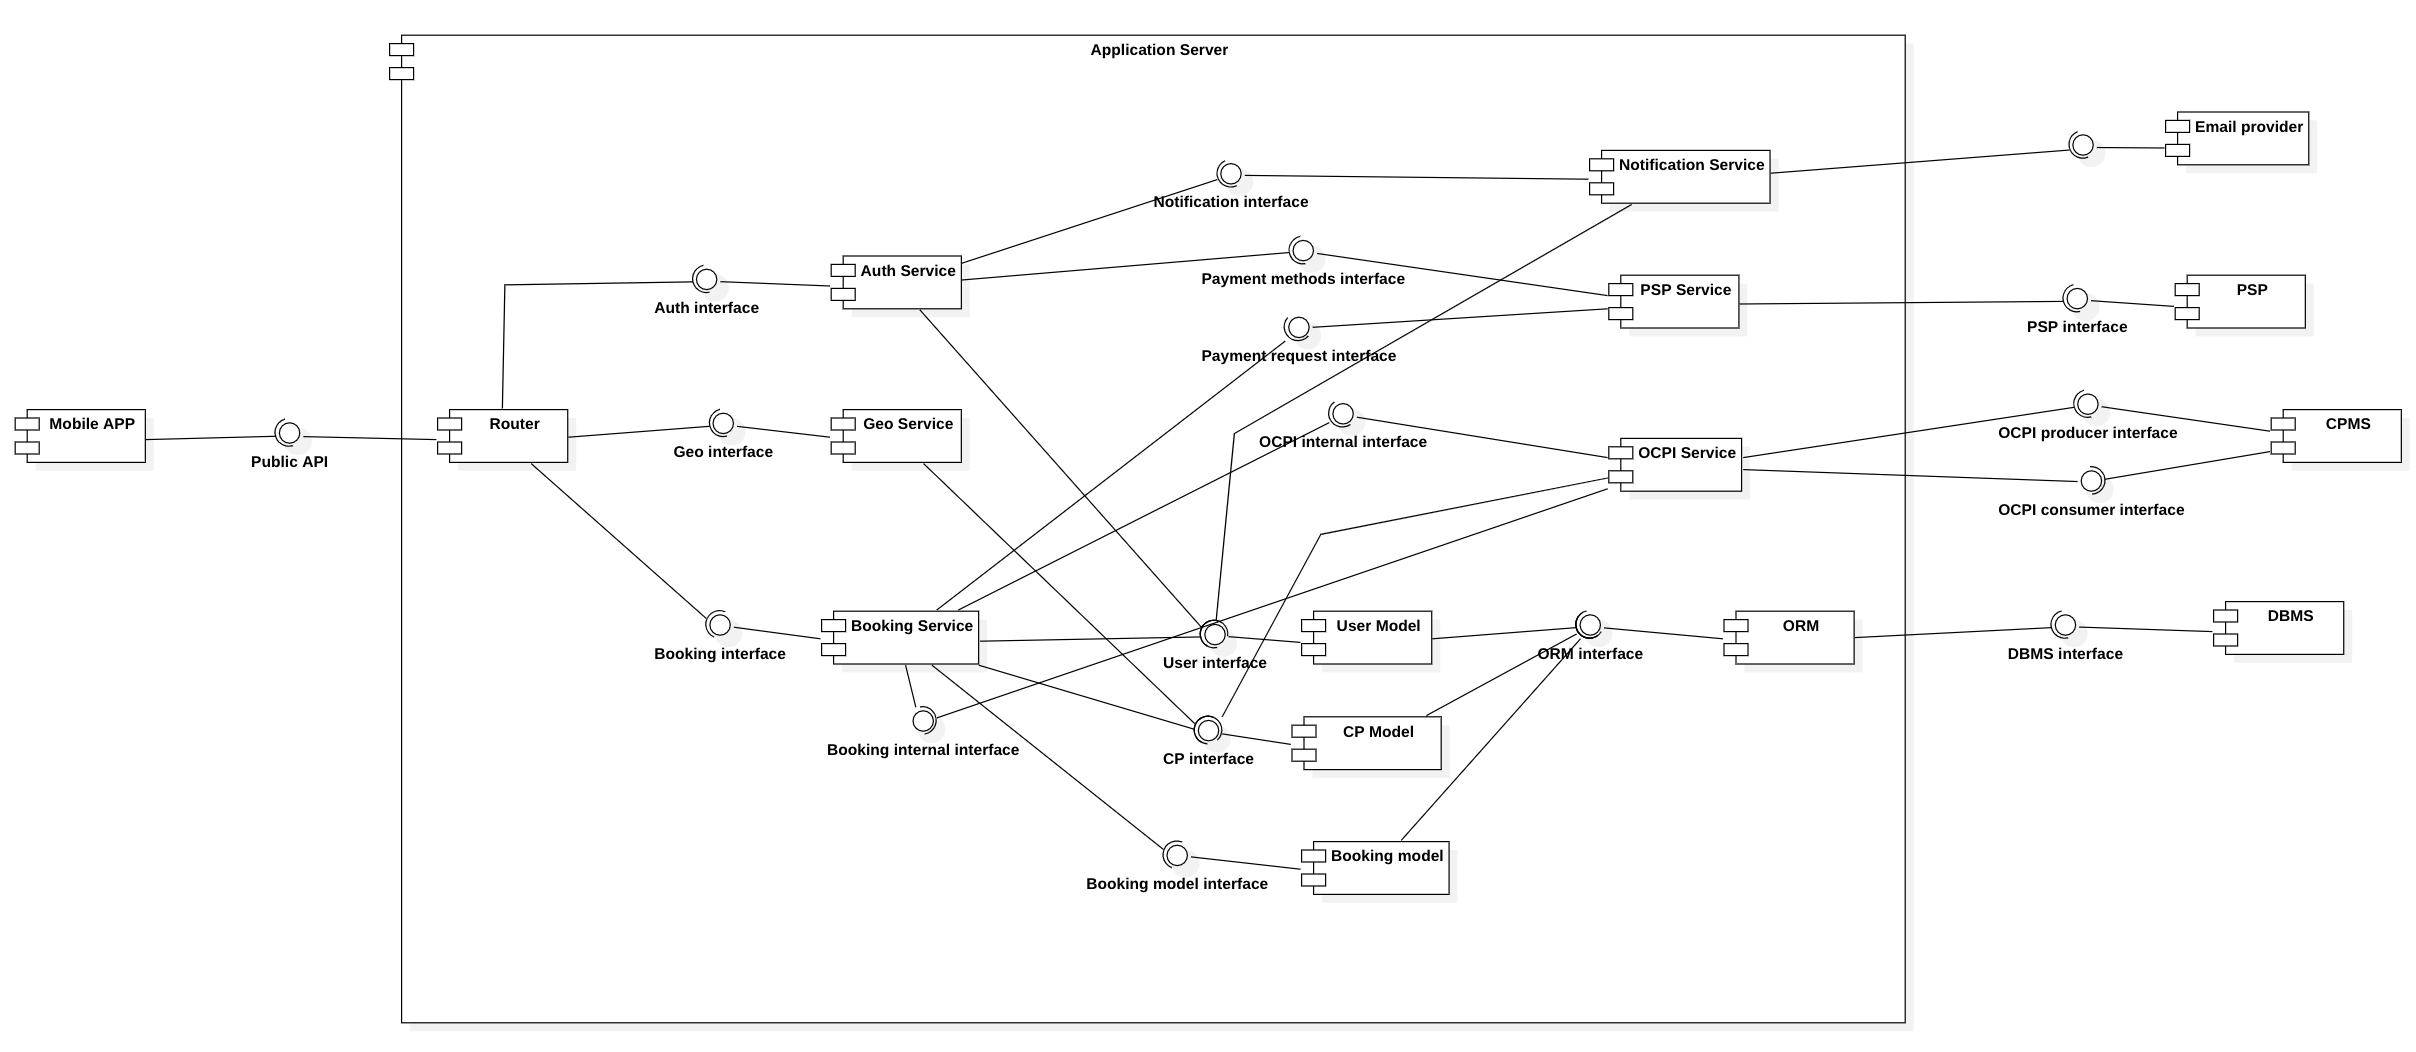
\includegraphics[angle=90,origin=c,height=14cm]{component_diagrams/component_diagram}
\caption{Component diagram of the system}
\end{figure}

\clearpage
\newpage

\begin{itemize}
	\item \textbf{Application server}: not a real "component" it shows the division between the backend, the frontend, the data layer and the external service. In the three-tier architecture it represents the Application layer.
	\item \textbf{Mobile APP}: mobile application for the system, used by the users.
	\item \textbf{Router}: handles all the requests directed to the Application APIs (i.e. OCPI PUSH endpoints are not handled here) that comes into the Application Server, uses the Auth Service to Authenticate and Authorize them. After that, if all the checks are passed, it will forward the request to the correct service that exposes the required route. It basically acts as a middleware, its presence is useful as it acts as a single point to develop all the authentication/authorization logic so that if it needs changes we can just update the router (and eventually the auth service) instead of updating all the services.
	\item \textbf{Auth Service}: is an internal service that handles authentication (Signup and login) and authorization (even if at the moment our system does not need that). It is mainly used internally but it exposes a couple of endpoints to the router for both signup and login.
	\item \textbf{Geo Service}: an highly reusable service, it uses a set of geographical points and exposes functionalities to list, filter and search those points based on their position. For our system is needed for the map functionality of the Mobile APP.
	\item \textbf{Booking Service}: it manages the booking for the application, it exposes some endpoints to the router for the booking functionalities of the Mobile APP and it is also used from other internal services.
	\item \textbf{Notification Service}: it manages all the notifications that the system needs to send to the user, both via email as via push services (e.g. Firebase Cloud Messaging)
	\item \textbf{PSP Service}: it manages the communication with the Payment Service Providers, it is useful as we can easily swap it with proprietary SDKs from the various providers.
	\item \textbf{OCPI Service}: it manages the communication with the CPMS, it exposes the endpoints for the PUSH part of the protocol (is needed to receive real-time updated from CPMS)
	\item \textbf{ORM}: a library that allows an easy to use mapping between Models and DB table, it handles queries and relationships. It is not worth it to develop an in-house solution, so we will use a library for that.
	\item \textbf{User Model, CP Model, Booking Model}: Models components that sit between services and ORM, useful to attach event listeners and other effects that need to run when updating the data. 
	\item \textbf{Email Provider}: external service (or services) that exposes API to send emails
	\item \textbf{PSP}: external service that exposes API to process payment
	\item \textbf{CPMS}: Charging Point Management System that exposes OCPI compliant API
	\item \textbf{DBMS}: Database Management System
\end{itemize}




















